\documentclass{article}
\usepackage{fullpage}
\usepackage[utf8]{inputenc}
\usepackage{graphicx}
\usepackage{hyperref}
\usepackage{tabularx}
\usepackage{attachfile}
\usepackage{pdfpages}
\usepackage{siunitx}
\usepackage{caption} \captionsetup[table]{skip=10pt}
\usepackage{graphicx}
\usepackage{subfig}
\usepackage{float}
\usepackage[nottoc,numbib]{tocbibind}

\title{Basic Lab Course 1: Pohl's Wheel (POR)}
\author{Technical University of Munich\\\\Leon Heiß, Paul Hildebrandt \\
Course 5, Group 7, Team 19}
\date{28. June 2022}
\begin{document}
\maketitle
\large
\begin{center}
\textbf{Abstract}\\
\normalsize
\medskip
In this experiment, the behaviour of a torsion pendulum, called the Pohl's Wheel, is examined. We first determine the natural frequency and the damping coefficient by means of a free damped oscillation, followed by evaluating the resonance frequency using forced oscillations with different excitation frequencies.
\end{center}
\normalsize
\tableofcontents
\newpage
\section{Theory}
\subsection{Free damped oscillation}
If a non-driven pendulum undergoes a damped oscillation around its resting position, this is called the damped natural oscillation of the system. The general equation of motion of the damped natural oscillation is \cite{1}:
\begin{equation}
    \Theta \ddot{\varphi}+\gamma \dot{\varphi} + k\varphi = 0.
\end{equation}
Here $\Theta$ is the moment of inertia of the pendulum, $\varphi$ is the deflection, $\gamma$ is the damping moment and $k$ is the restoring moment of the spring. For the pendulum used in the experiment, it makes sense to introduce the damping coefficient $\lambda = \gamma \cdot \Theta /2$. In addition, only the oscillation case is considered, i.e. the one which occurs when the pendulum is weakly damped: $\lambda^2 < k/\Theta$. In this case, the solution for the equation of motion is:
\begin{equation}
    \varphi(t)= \varphi_0 \cdot \textrm{exp}(-\lambda t) \cdot \textrm{exp}[i(\omega_d t + \delta)],
\end{equation}
with $\varphi_0$ being the resting position of the systems, $\delta$ the phase shift and $\omega_d = \sqrt{\frac{k}{\Theta}-\lambda^2}$ being the natural angular frequency of the damped oscillation. In reality, the solution corresponds to the real part, i.e
\begin{equation}
    \varphi(t)= \varphi_0 \cdot \textrm{exp}(-\lambda t) \cdot \cos(\omega_d t + \delta).
\end{equation}
The cosine term describes the oscillation and the exponential term describes the damping, i.e. the envelope of the amplitude. This oscillation can be characterized by the decay time $\tau$
\begin{equation}
    \tau = \frac{1}{\lambda},
\end{equation}
and the natural frequency $f$
\begin{equation}
    f = \frac{\omega_d}{2 \pi}.
\end{equation} 
The resulting function is shown in Figure 1.
\begin{figure}[hbt!]
\centering
\includegraphics[width=300pt]{dämpfung-theory.png}
\caption{Real part of the oscillation for weak damping, amplitude versus time. \cite{1}}
\label{fig:length_eight_mouse}
\end{figure}
\subsection{Resonance curve}
If an external drive applies additional torque to the pendulum, Equation 1 changes to:
\begin{equation}
    \Theta \ddot{\varphi} + \gamma \dot{\varphi} + k\varphi = M_0 \cdot \sin(\omega t).
\end{equation}
If we insert the particulate solution
\begin{equation}
    \varphi_{p}(t)= A(\omega)\cdot \sin(\omega t - \delta)
\end{equation}
into Equation 6, we can determine the amplitude function $A(\omega)$\cite{1} as
\begin{equation}
    A(\omega)= \frac{\frac{M_0}{\Theta}}{\sqrt{(\omega_{0}^2 -\omega^2)^2+4\lambda^2 \omega^2}},
\end{equation}
with $\omega$ being the driving frequency and $\omega_0 = \sqrt{\frac{k}{\Theta}}$ the natural frequency of the freely swinging pendulum. Equation 8 reaches its maximum value at the so-called resonance frequency
\begin{equation}
    \omega_R= \sqrt{\frac{k}{\Theta}-2\lambda^2},
\end{equation}
which can be determined using
\begin{equation}
    A(\omega_R)= \frac{M_0}{2\Theta \cdot \lambda \cdot \omega_d}.
\end{equation}
If we plot the graph of $A(\omega)$, as seen in Figure 2, we can see that the resonance curve is not symmetric with respect to $\omega_R$.
\begin{figure}[hbt!]
\centering
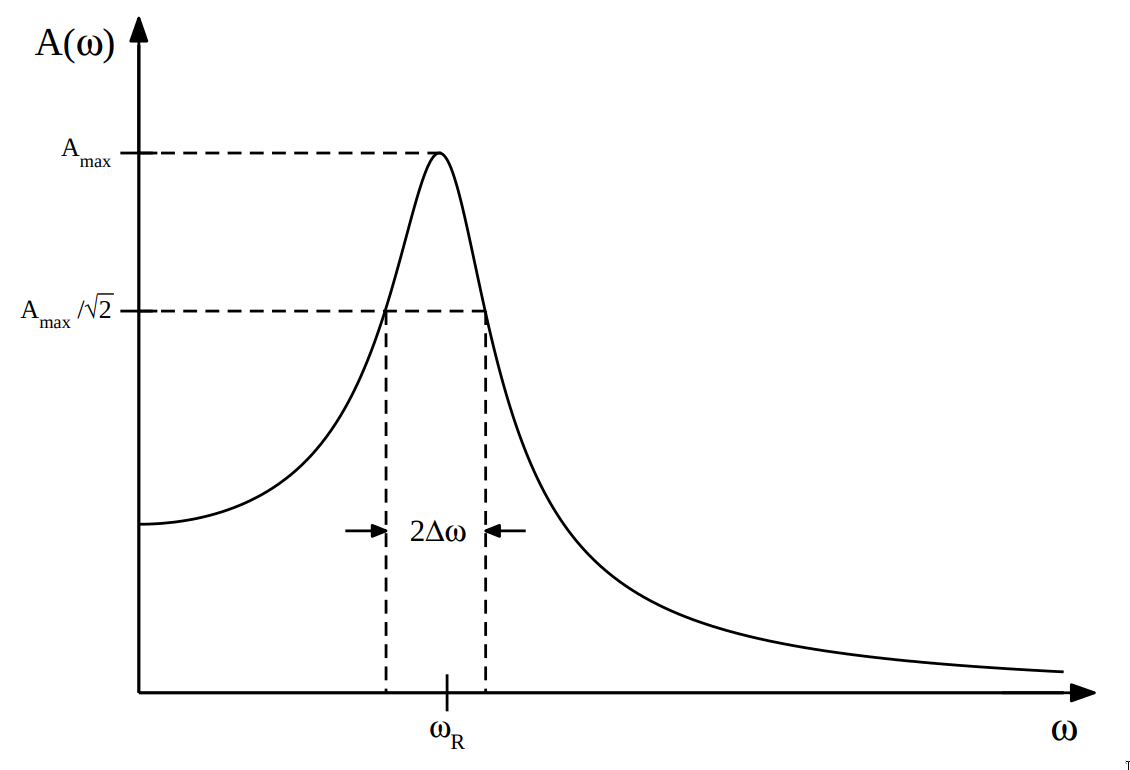
\includegraphics[width=350pt]{res-theory.png}
\caption{Resonance curve with marked full width at half maximum. \cite{1}}
\label{fig:length_eight_mouse}
\end{figure}
The so-called full width at half maximum (FWHM) is the width of the resonance curve measured between those points on the y-axis which are half the maximum amplitude. We can determine $\Delta \omega$ around $\omega_R$ by measuring half the difference between those $\omega$ values that are present at $\frac{A(\omega_R)}{\sqrt{2}}$. For small damping coefficients $\lambda$, the following relationship also applies:
\begin{equation}
    \Delta \omega= \lambda.
\end{equation}
From Equation 11 we can observe that the FWHM increases/decreases as the damping increases/decreases. In addition, the lifespan of the oscillation increases as $\lambda$ decreases.
\section{Experimental setup}
The torsional pendulum, or Pohl's Wheel, consists of a circular copper ring with an eddy current brake, and a spiral spring.
One end of the spring is attached to the copper ring, to hold it in a resting position, the other end to a motor via an eccentric rod mechanism.
The ring also features a circular scale which is used to read of the deflection. Different levels of damping can be selected by controlling the current through the eddy current brake.
\begin{figure}[hbt!]
\centering
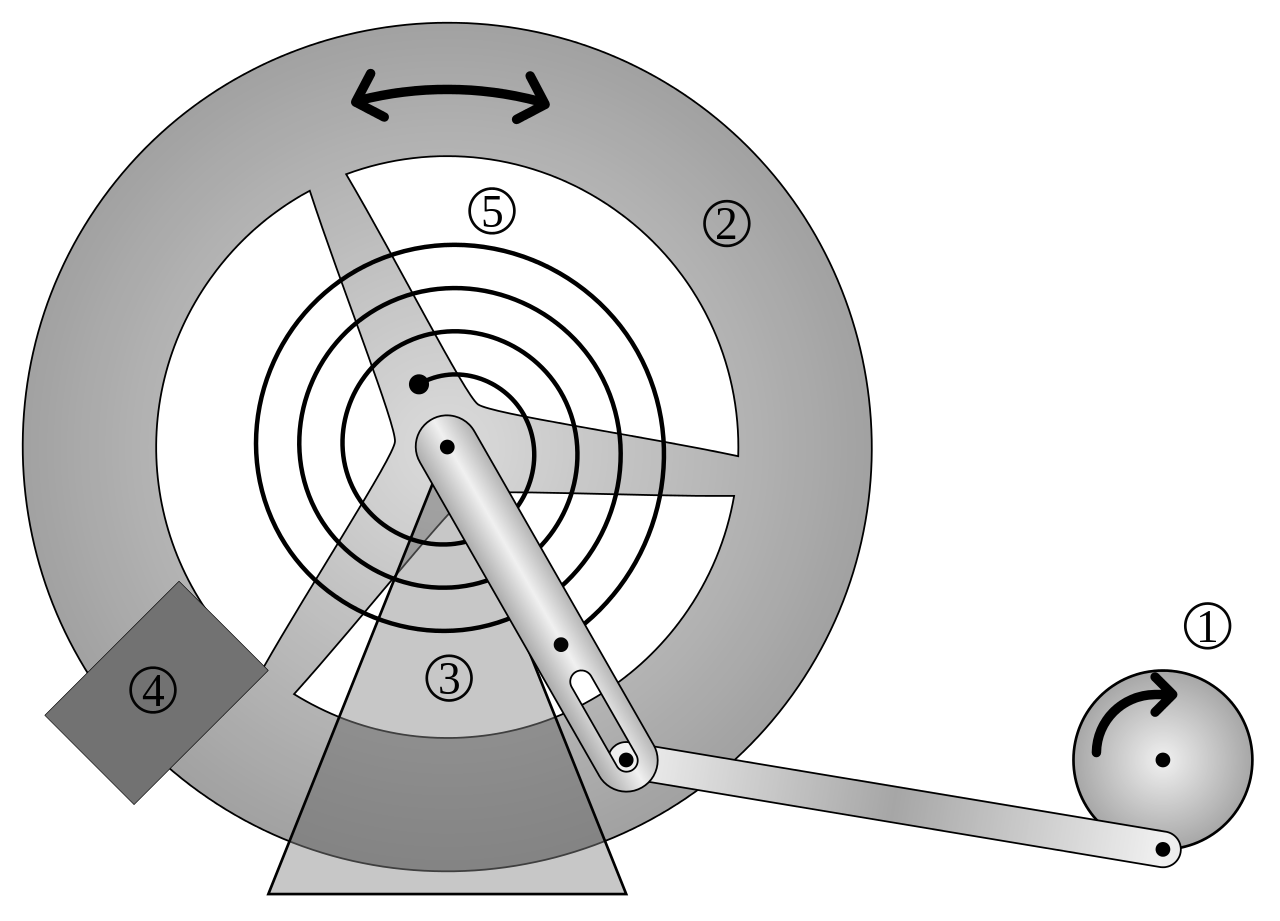
\includegraphics[width=250pt]{rad.png}
\caption{Pohl's Wheel: (1) motor, (2) pendulum, (3) bearing, (4) eddy current brake, (5) spiral spring. \cite{3}}
\label{fig:length_eight_mouse}
\end{figure}
\section{Damping coefficient}
In Theory, the damping force by the eddy current can be described with \cite{1}
\begin{equation}
	F \propto v \cdot B^2
\end{equation}
and thereby
\begin{equation}
	\lambda \propto I^2.
\end{equation}
These relations will now be tested experimentally.
\newpage
\subsection{Constant current}
The most simple case of a damped oscillation was already described in equation 3.
$\lambda$ is constant in case the current is.
In our first setup, 0,45(0,01)A flow through the electromagnet.
As the dampening effect creates an enveloping function for the oscillation, the amplitude of the peaks in positive and negative direction are directly affected.
In order to determine the time between two maxima, the arithmetic mean of five measurements of the duration of ten periods is taken and divided by ten.
The according calculations are further discussed in section 4.1.
This approach does not take into account that the angular velocity changes with the amplitude.
Since measuring the amplitude by sight is quite inaccurate ($\pm 0,036$ or 2,5$\%$ of the maximal amplitude) anyway, this can be neglected.
By plotting the amplitude semi-logarithmically, a straight line can be drawn through these points.
The slope of the natural logarithm of this line is $-\lambda$ (figure 4).
\begin{figure}[hbt!]
\centering
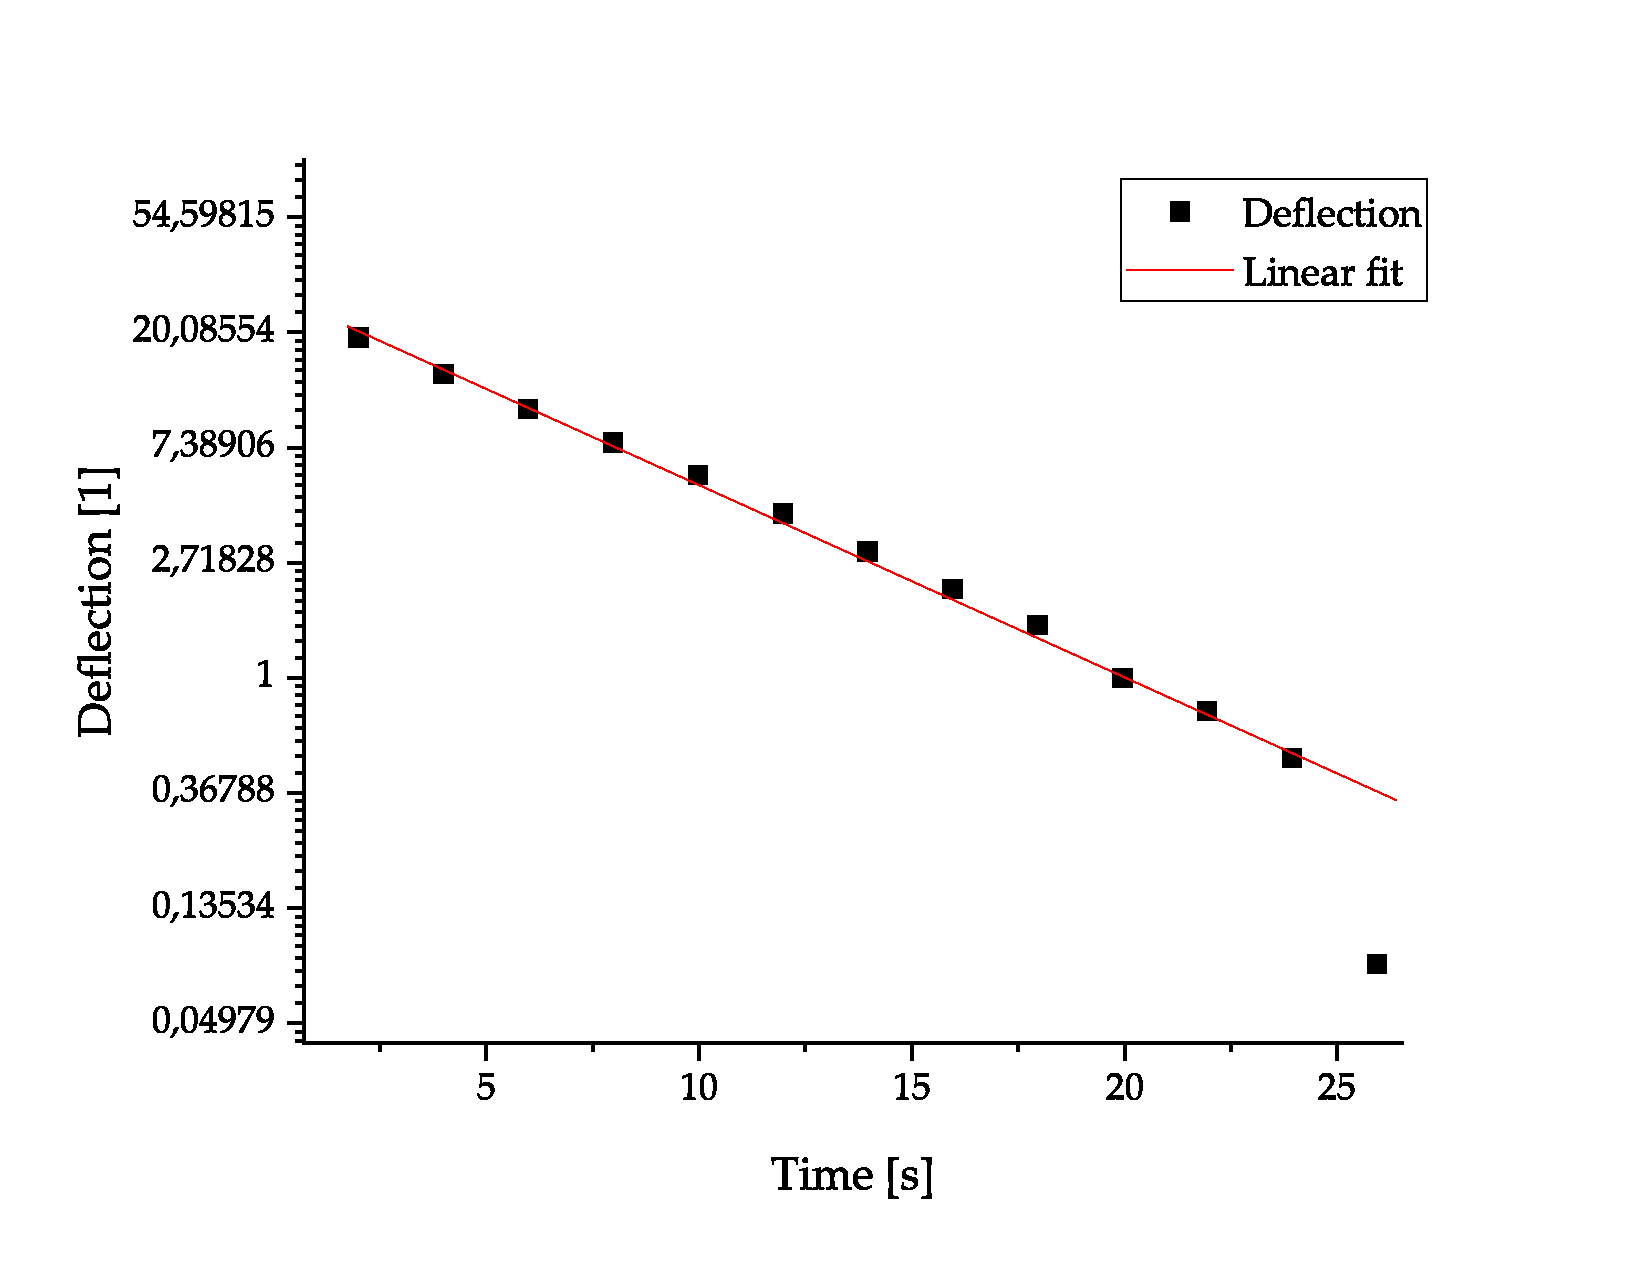
\includegraphics[width=400pt]{manualPlot.eps}
\caption{Semi logarithmic plot of peak amplitude with linear fit. (Manually recorded data)}
\label{fig:length_eight_mouse}
\end{figure}
The same measurement was performed using a digital measurement method (figure 5).
\begin{figure}[H]
\centering
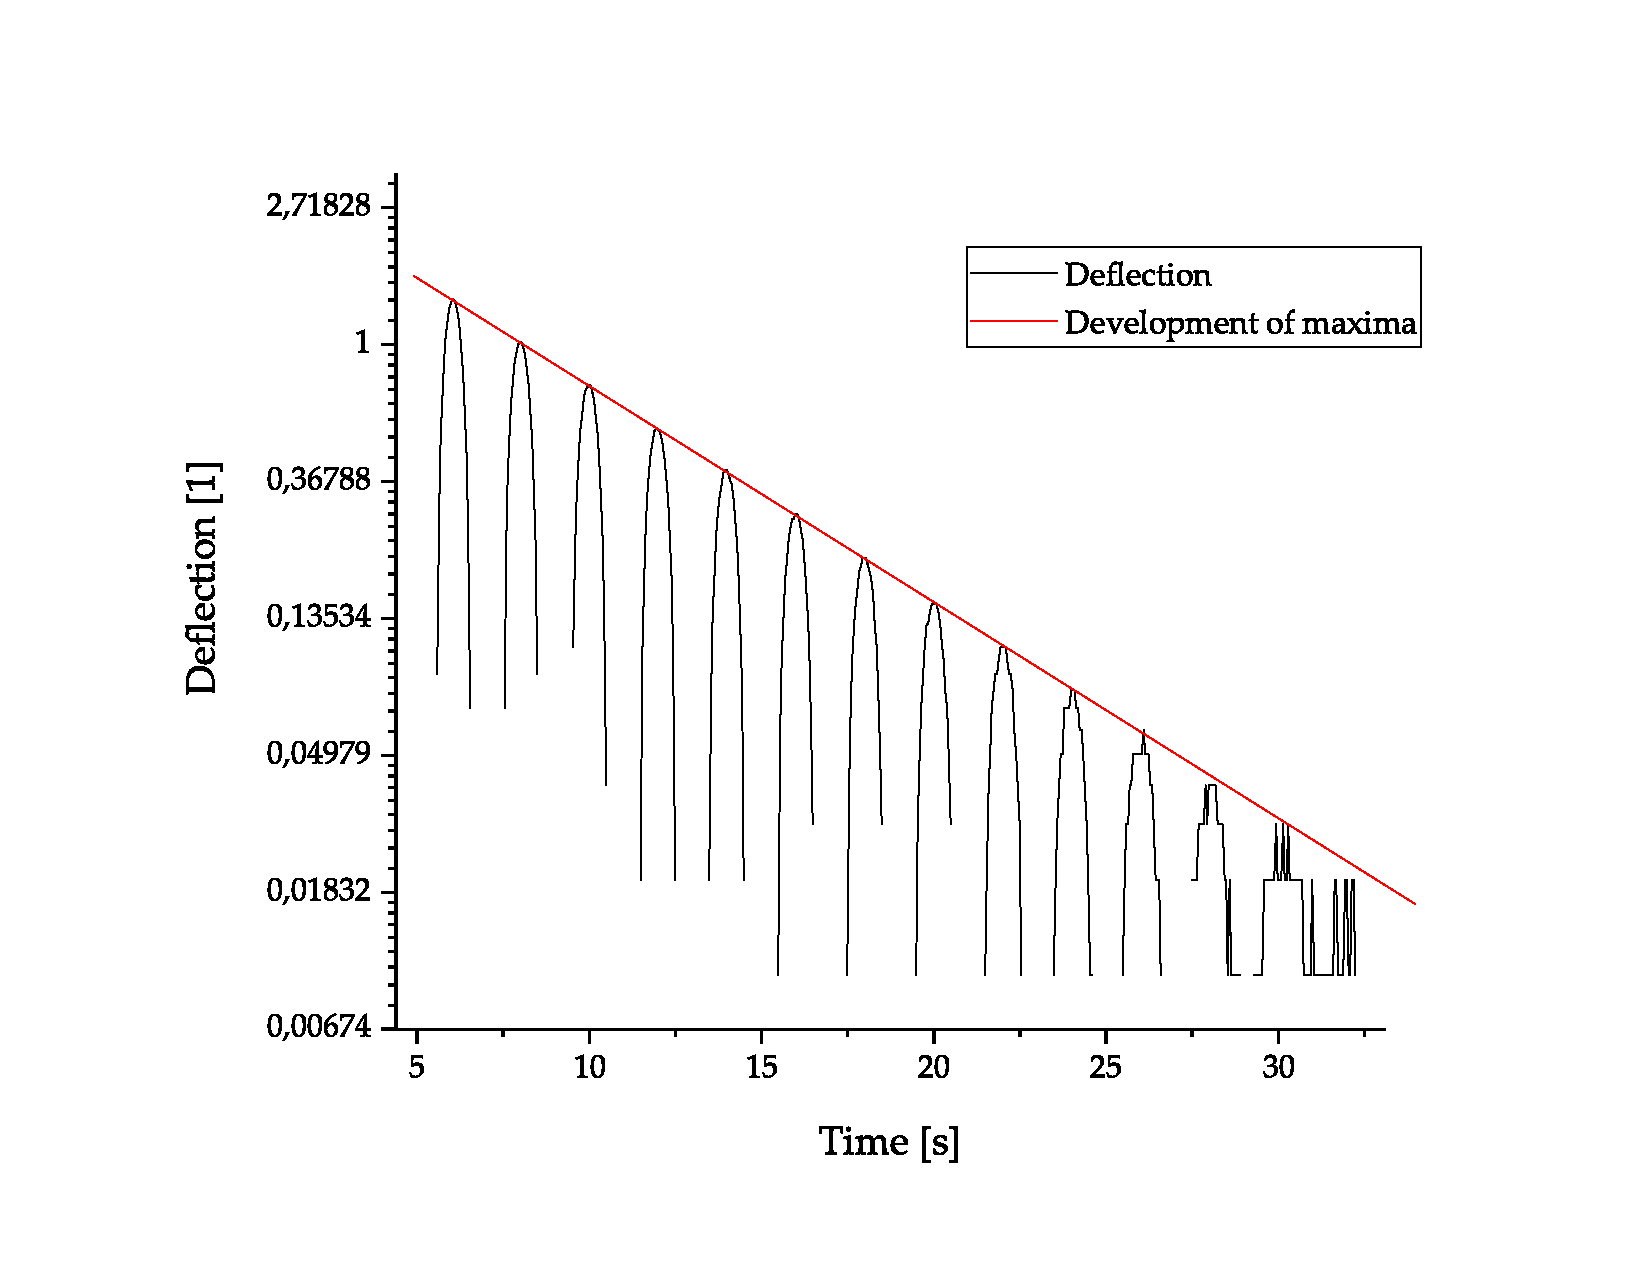
\includegraphics[width=350pt]{CD1-L-E.eps}
\caption{Semi logarithmic plot of peak amplitude with linear fit. (Digitally recorded data)}
\label{fig:length_eight_mouse}
\end{figure}
The resulting data deviates only slightly:\\
\begin{table}[H]
\caption{Damping coefficient $\lambda$ and decay time $\tau$ for 0,45A; measured manually and by computer.}
\centering
\begin{tabular}{|c|c|c|}
\hline 
  & Computer & Manually \\ 
\hline 
$\lambda$ & 0,157(0,010) & 0,161(0,036) \\ 
\hline 
$\tau$ & 6,098(0,406) & 6,227(1,396) \\ 
\hline 
\end{tabular}
\end{table}
\noindent
Note that both measurements use a different scale. This has no further effects on the evaluation since it only acts as a constant factor for the amplitude.
The manual measurement has a higher uncertainty. These values had to be estimated during a very short timespan. This uncertainty propagates to the values $\lambda$ and $\tau$. Still, the results are close and lie within each others area of uncertainty.
\subsection{Behaviour at varying current}
As a next step, the influence of the current on angular velocity $\omega$ and the damping coefficient $\lambda$ is examined.
Due to its precision and efficiency, only digitally recorded data is used. The curves are fitted with the standard equation for damped oscillations (3) which can be seen in figure 6.
\nopagebreak
\begin{figure}[H]
\centering
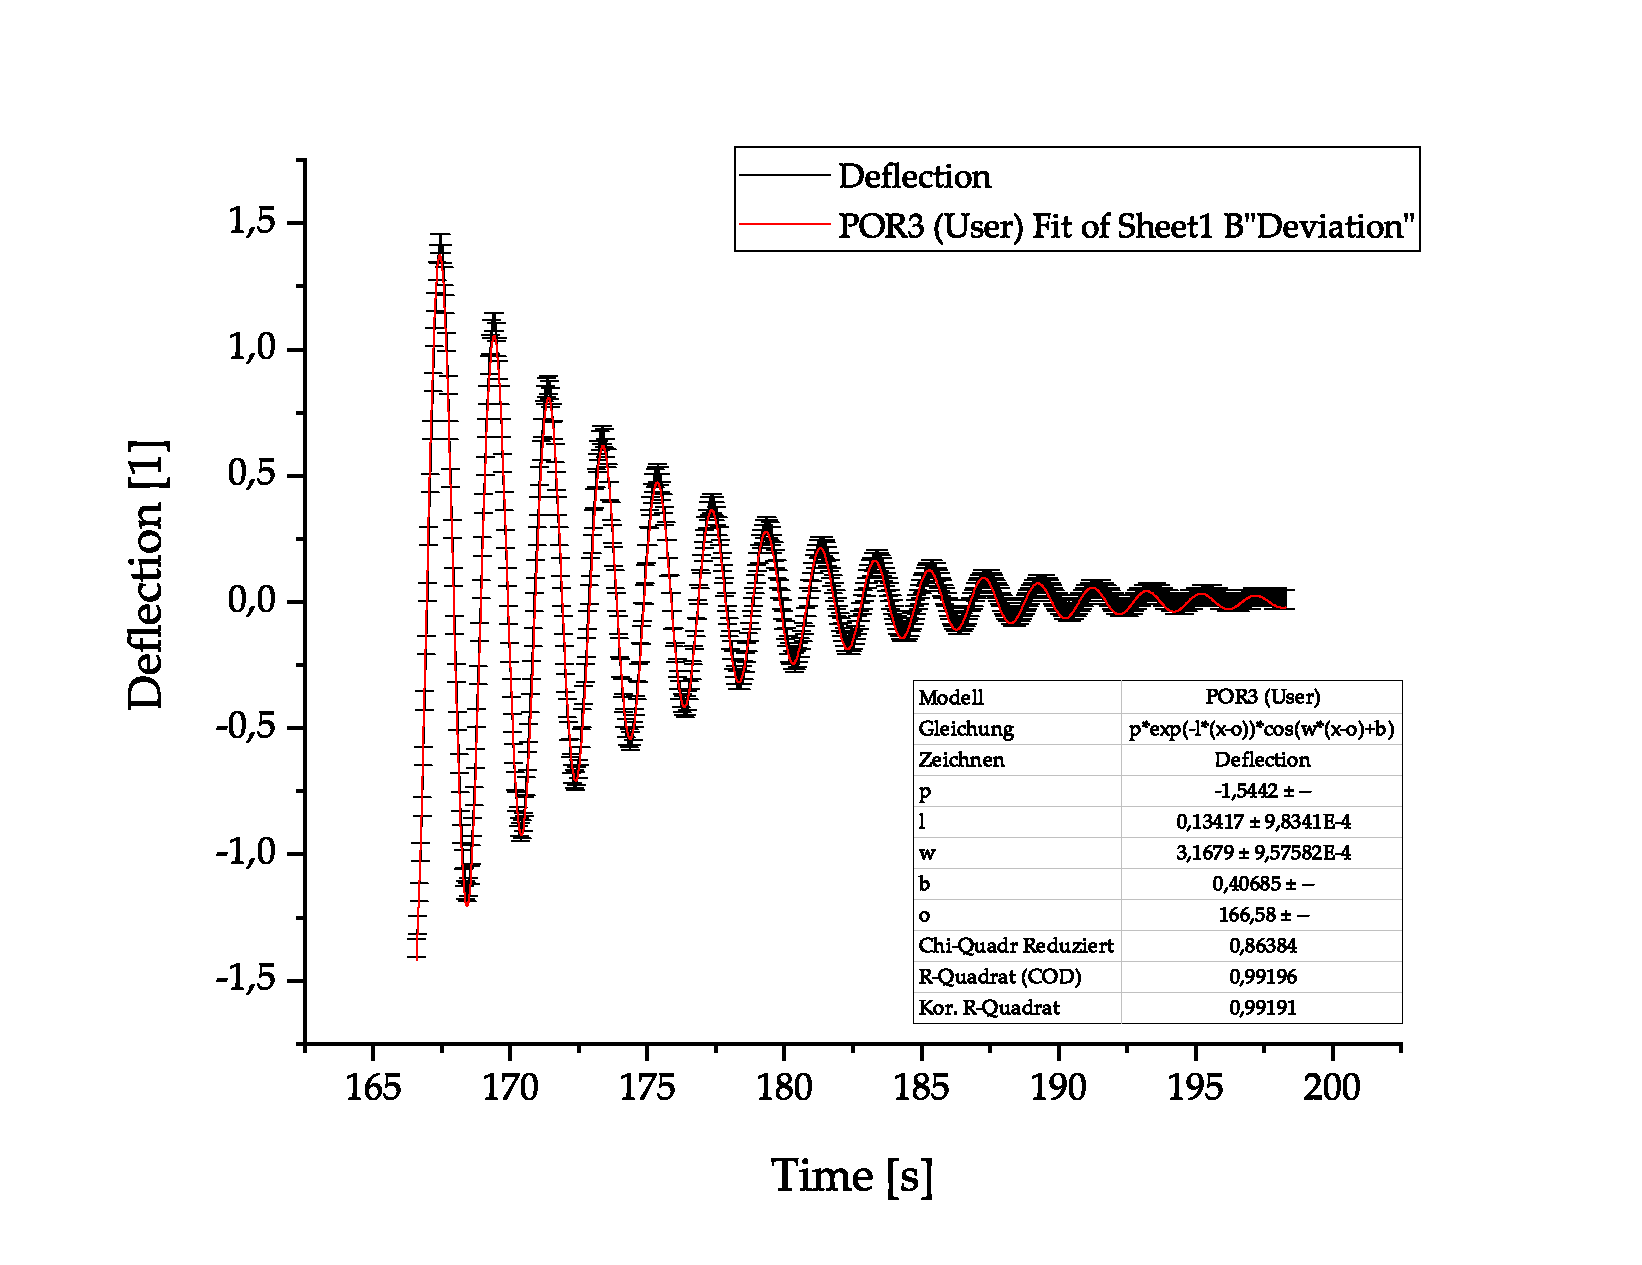
\includegraphics[width=350pt]{0-4A.eps}
\caption{Oscillation with 0,4A damping current and according fit.}
\label{fig:length_eight_mouse}
\end{figure}
\nopagebreak
\noindent
The shift in frequency with changing amplitude is not taken into account for the fitting function. A slight resulting deviation can be observed in figure 6. This fit is performed for all data for currents from 0,2A up to 1,5A with 0,1A increment. The resulting plot is shown in figure 7.
As seen, the expected quadratic growth from equation (13) is met.
We also obtain information about the angular velocity from the fits, shown in figure 8.
One can observe that the theoretical curve
\begin{equation}
\omega(I) = \sqrt{\frac{k}{\theta}-2\cdot\lambda(I)^2}
\end{equation}
does fit the data. Taking into account that the uncertainty bars are referring to a 1-$\sigma$ interval, about every third points bar should be outside the theory curve, which is met.
It can be concluded that equation (12) and (13) are valid for this experimental setup.
\nopagebreak
\begin{figure}[H]
\centering
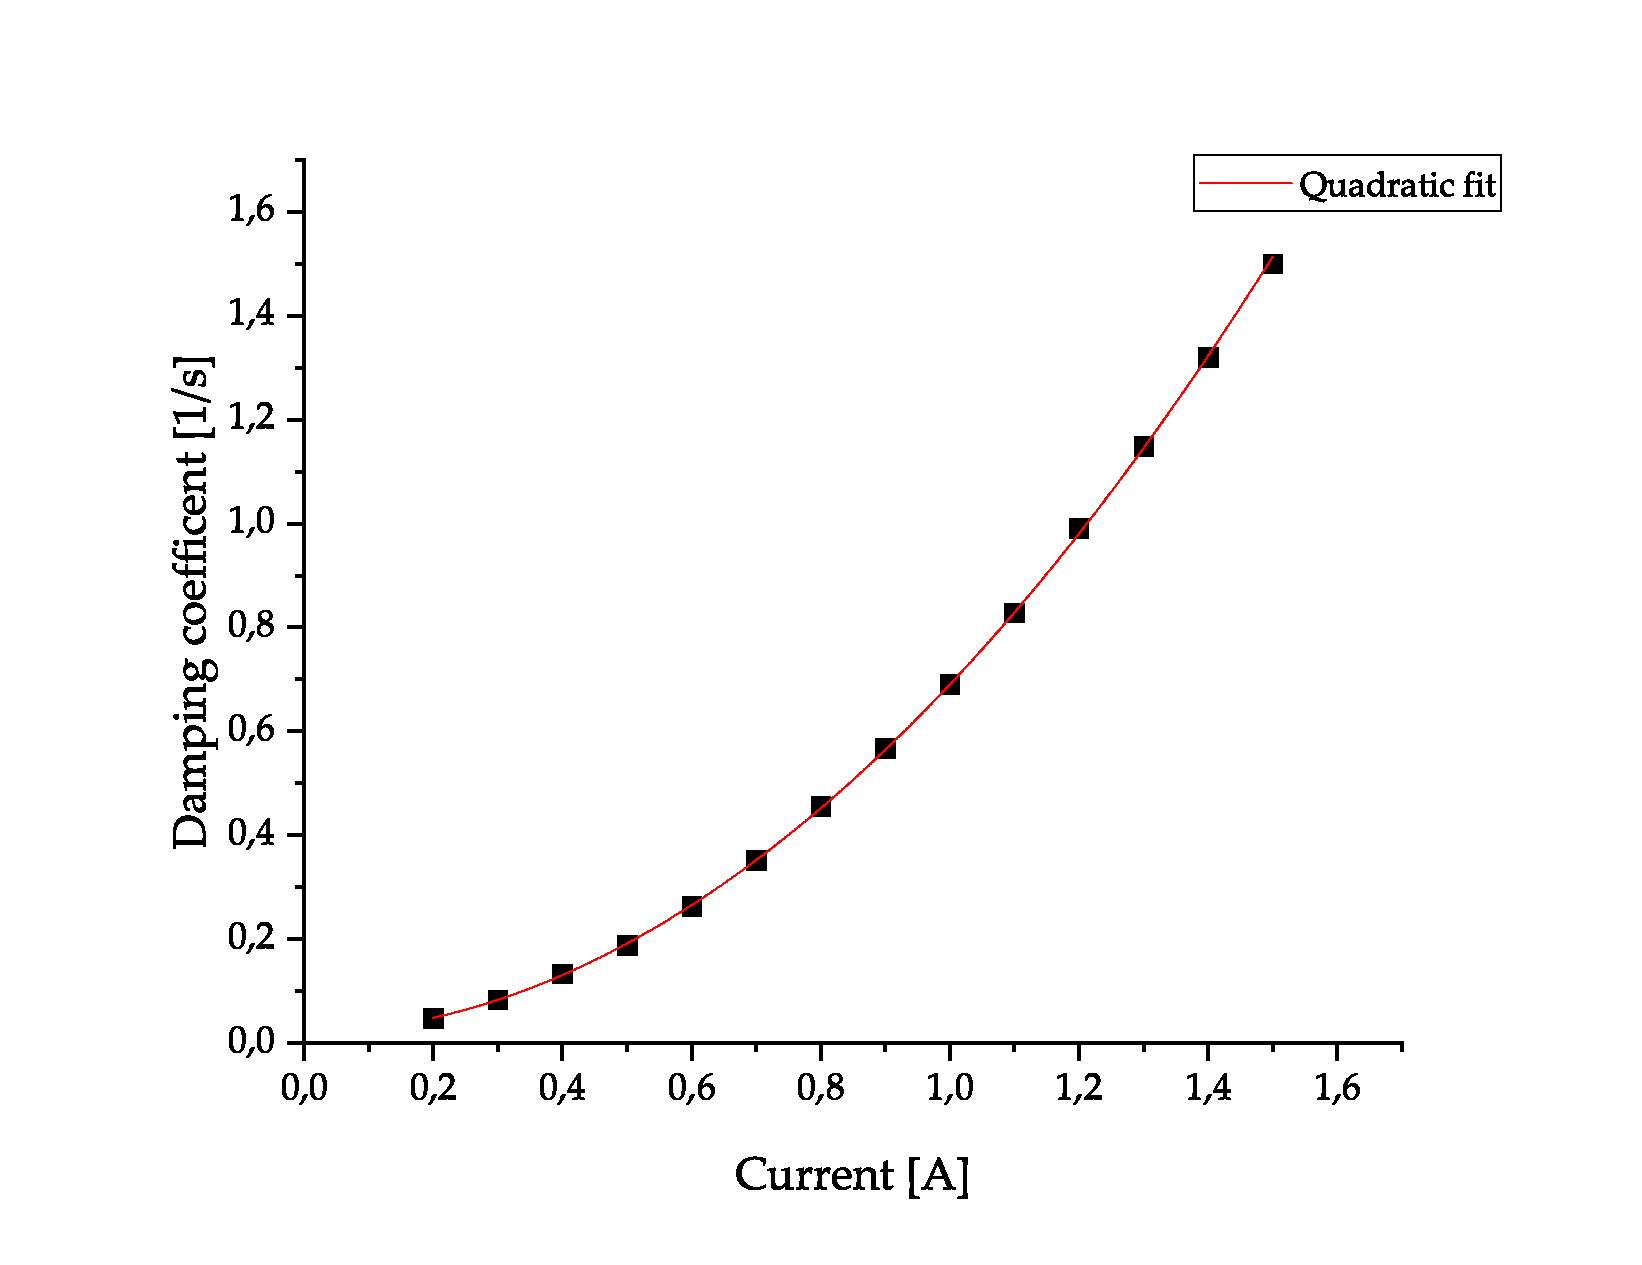
\includegraphics[width=320pt]{damping.eps}
\caption{Damping coefficients for different currents and according quadratic fit.}
\label{fig:length_eight_mouse}
\end{figure}
\begin{figure}[H]
\centering
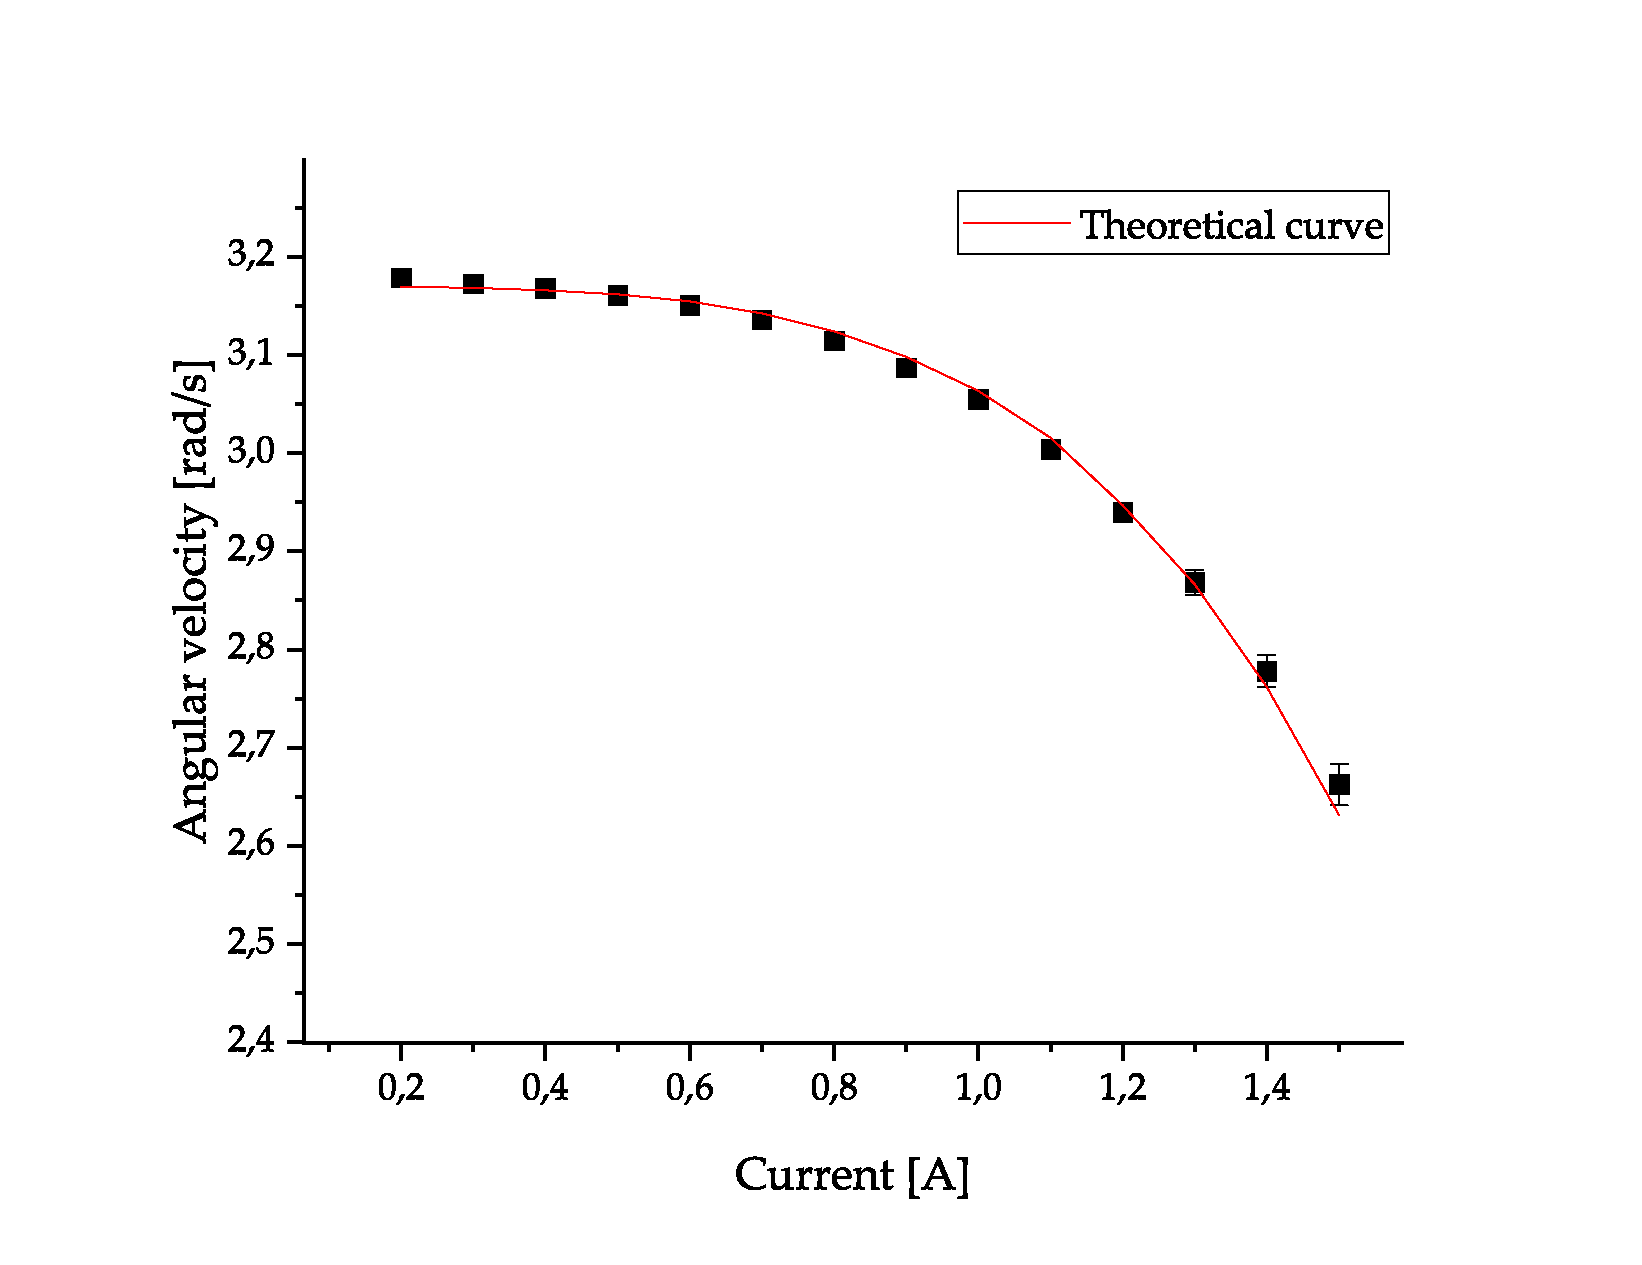
\includegraphics[width=320pt]{frequency.eps}
\caption{Natural frequency for different currents and according theoretical curve.}
\label{fig:length_eight_mouse}
\end{figure}
\section{Natural frequency}
\subsection{Behaviour at constant damping rate}
To determine the natural frequency of the torsional pendulum at a constant damping rate, we measure the time it takes for the pendulum to undergo 10 full oscillations.
At first this is done manually by using a stopwatch, followed by a more precise digital measurement using the computer.
In both cases we use a constant damping current of $0.45 \pm 0.01$ A.
For the plot, the arithmetic mean of three measurements for the amplitude is calculated.
\begin{table}[H]
\caption{Manual measurements with stopwatch.}
\centering
\begin{tabular}{| >{\centering\arraybackslash}m{2cm} | >{\centering\arraybackslash}m{5cm} |}
\hline
\rule{0pt}{5pt}
Attempt & Time for 10 oscillations $T_{10}$ [s]  \\ \hline
 1 & 19.96  \\ \hline
 2 & 19.86 \\ \hline
 3 & 19.93 \\ \hline
 4 & 19.97 \\ \hline
 5 & 19.99 \\ \hline
\end{tabular}
\end{table}
\noindent
We can calculate the period $T$ with:
\begin{equation}
    T = \frac{T_{10}}{10},
\end{equation}
where $T_{10}$ is the time needed for 10 oscillations. By taking the mean of the 5 measurements we get $T_{10} = 19.942$ s and period $T=1.994 \pm 0.05$ s. For the uncertainty of the period, which comes from the human starting and stopping the stopwatch, we assumed an average reaction time of 250ms. We can now use the relationship
\begin{equation}
    \omega_d = \frac{2\pi}{T}
\end{equation}
for the natural angular frequency, which comes to $\omega_{d} = 3.151 \pm 0.079$ s$^{-1}$, to determine the natural frequency $f$ with Equation 5. For the manual measurements we come to the natural frequency $f = 0.501 \pm 0.018$ Hz. The same is then repeated for the digital measurements (Figure 9), we obtain $T=1.986 \pm 0.01$ s,  $\omega_{d} = 3.164 \pm 0.016$ s$^{-1}$ and  $f = 0.503 \pm 0.004 $ Hz.
\begin{figure}[H]
\centering
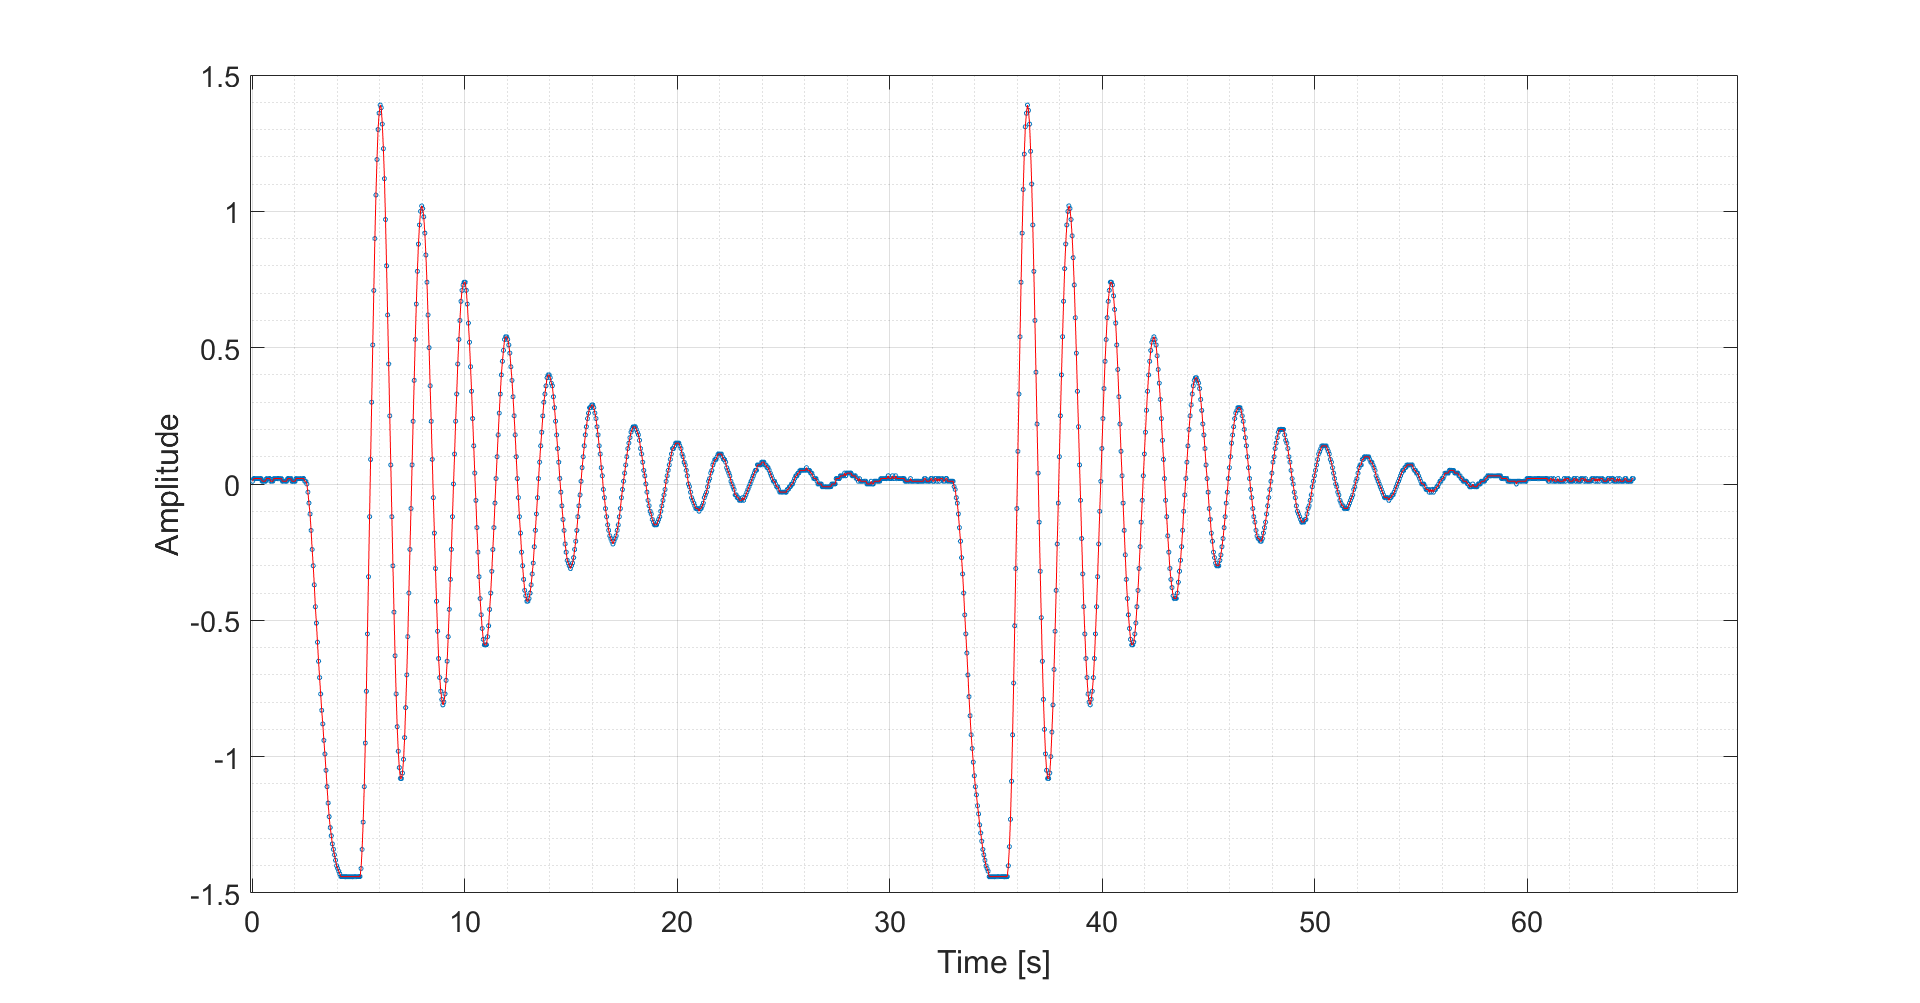
\includegraphics[width=400pt]{eigen.png}
\caption{Digital measurements for natural frequency, amplitude vs time.}
\label{fig:length_eight_mouse}
\end{figure}
\subsection{Behaviour at varying damping rate}
As already seen in equation (9), the natural frequency depends on the dampening constant.	Similar to figure 8, we obtain figure 10:
\begin{figure}[H]
\centering
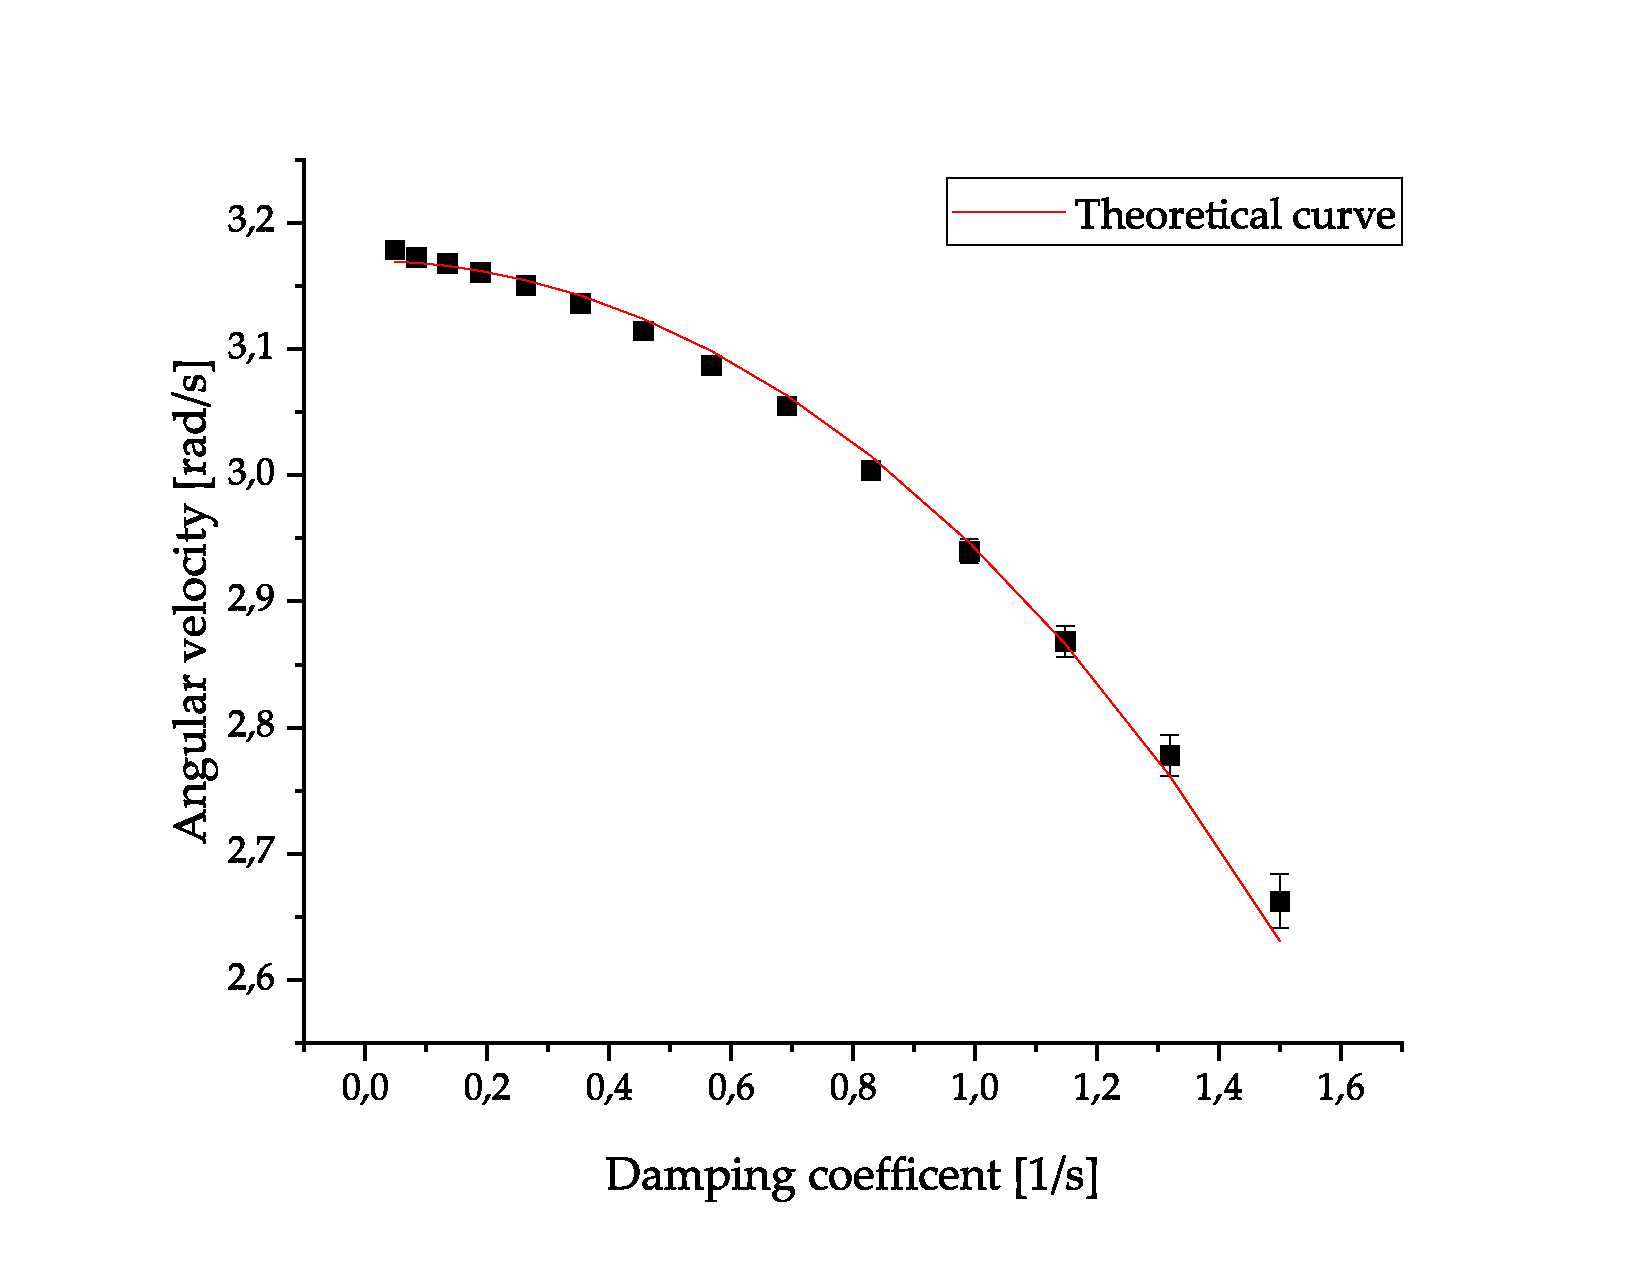
\includegraphics[width=350pt]{DampeningVsFrq.eps}
\caption{Natural frequency of damping coefficients with theoretical curve.}
\label{fig:length_eight_mouse}
\end{figure}
\noindent
Figure 10 also contains points that closely fit the theoretical curve.
\section{Resonance curve}
In order to determine the resonance frequency and curve of the pendulum, we measure the amplitudes at varying excitation frequencies using the motor. We start off with steps of 100 Hz on the function generator and increase from there. During those measurements we plot the values ourselves on a piece of paper to roughly estimate where the resonance frequency lies. Closer to the resonance frequency we measured in steps of 50 Hz. As noted in the instructions \cite{1}, 3200 steps correspond to one revolution of the motor, so a frequency of 3200 Hz on the frequency generator corresponds to a excitation frequency of 1 Hz. If we plot the measured amplitudes against the excitation frequencies, we get the following graph:
\begin{figure}[H]
\centering
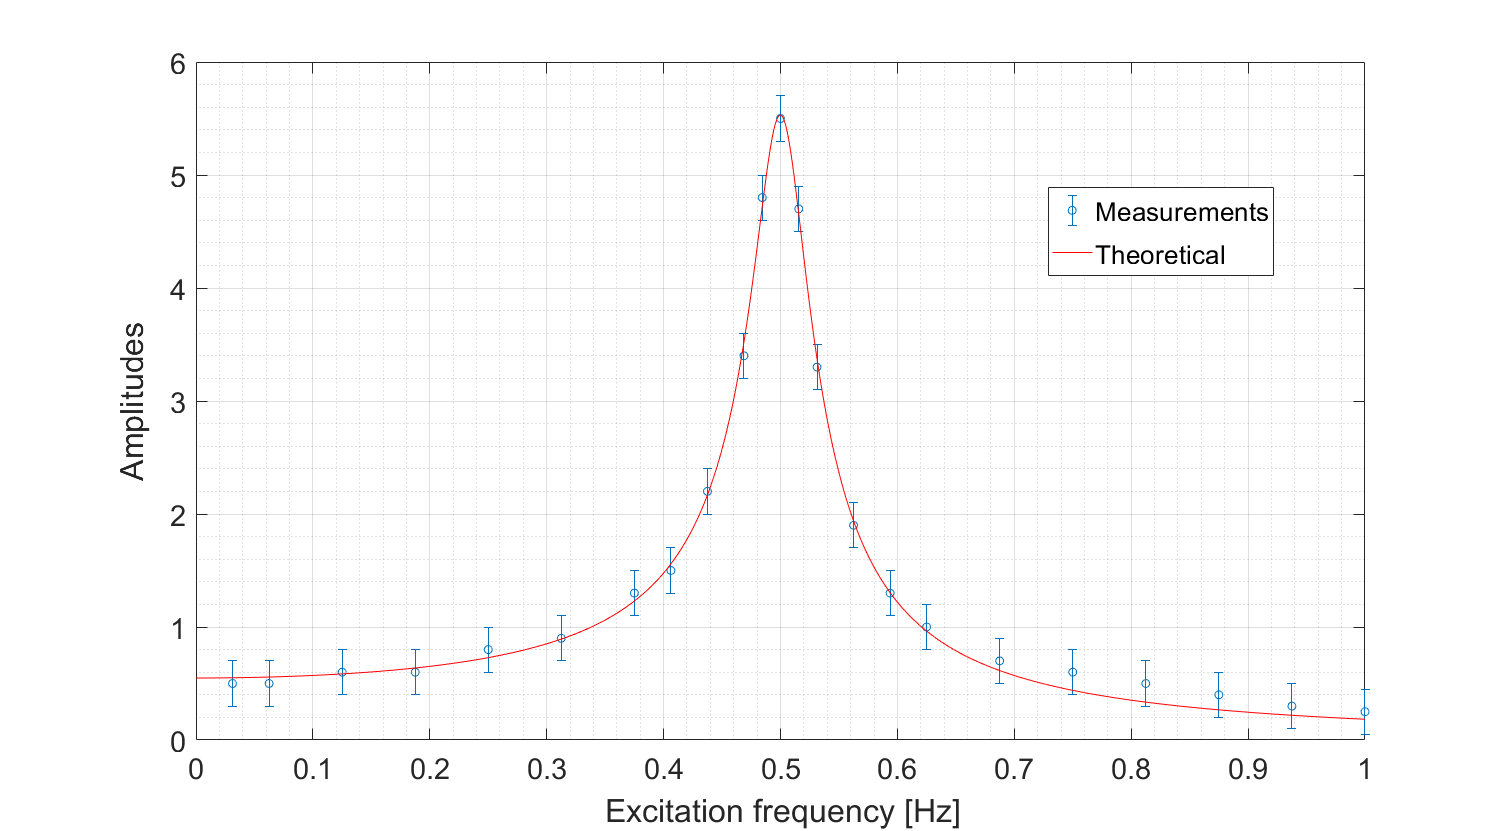
\includegraphics[width=470pt]{rescurve.png}
\caption{Resonance curve, amplitudes vs excitation frequency.}
\label{fig:length_eight_mouse}
\end{figure}
\noindent
Comparing it to the expected theoretical curve, which we obtained by performing a fit with Equation 8 using the free parameters $\omega_0, \lambda$ and $\frac{M_0}{\Theta}$, one can observe that our measurements are compatible within uncertainties with the expected values.
In order to precisely determine the resonance frequency, one derives Equation 8 with respect to $\omega$ and then sets it equal to zero. Solving for $\omega$, we get $\omega_R = 0.498 \pm 0.018$ s$^{-1}$.
The FWHM is obtained by substituting the value of $w_R$ into Equation 8. The result is then divided by $\sqrt{2}$ and the equation $A(\omega)$ is solved for $\omega$. The difference between the two resulting positive solutions is now equal to twice the full width at half maximum, which comes to $\Delta \omega = 0.1148 \pm 0.0168$ s$^{-1}$. According to Equation 11, $\Delta \omega$ should in theory match $\lambda$ since there is weak damping. In fact, the function fit in Matlab gives the value $\lambda = 0.125
 \pm 0.013 $. The value of $\lambda$ in the first part of the experiment also comes close to the measurement and just barely does not agree with $\Delta \omega$ within the uncertainties. We can safely conclude that relationship in Equation 11 is for the most part fulfilled and the deviations most likely came from an inaccurate measurement.
\begin{thebibliography}{9}
\bibitem{1}
Fakultät für Physik. \emph{Pohlsches Rad} (28.06.2022).
\textbf{URL:} \url{https://www.ph.tum.de/academics/org/labs/ap/ap1/POR.pdf}
\bibitem{2}
Fakultät für Physik. \emph{ABW-Skript} (28.06.2022).
\textbf{URL:} \url{https://www.ph.tum.de/academics/org/labs/ap/org/ABW.pdf}
\bibitem{3}
Georg Wiora. \emph{Prinzipzeichnung des Pohlschen Rades} (28.06.2022).
\textbf{URL:} \url{https://commons.wikimedia.org/wiki/File:Pohl_Wheel.svg}
\end{thebibliography}
\section{Appendix}
\subsection{Error estimation}
\paragraph{Damping coefficient}
Three error sources had to be taken into account: The multimeter measuring the current with $\pm$0,01A, the accuracy of reading the amplitude manually with 0,25 and the  accuracy of reading the amplitude digitally with 0,01. All errors were propagated using equation (18), (19) and (20) from the ABW-script \cite{2}. For all fits, an 1$\sigma$-uncertainty interval was chosen.
\paragraph{Natural frequency}
For the measurements of the natural frequency one source of error has to considered, which is the aforementioned time uncertainty that comes from starting and stopping the stopwatch, which we assumed to be around 250ms for each interaction. For the digital measurements using the computer, we used $u(T)=0.01$ s, as the setup only allowed us to recorded two significant digits. By using Gaussian error propagation we then come to an uncertainty of 
\begin{equation}
    u(f)= f \cdot \sqrt{\bigg(\frac{u(T)}{T}\bigg)^2+\bigg(\frac{u(\omega_d)}{\omega_d}\bigg)^2}.
\end{equation}

\paragraph{Resonance curve}
In theory two sources of error have to be considered for the resonance experiment, namely the reading accuracy of the amplitude and the uncertainty of the function generator, but as the uncertainty of the function generator is rather low, it can be safely neglected. For the reading uncertainty of the amplitude we chose $u(A) = 0.2$, which equals one step on the division scale. Similar to the uncertainty for the natural frequency we then used Gaussian error propagation to get the values for the resonance frequency and FWHM.
\subsection{Lab notebook} 
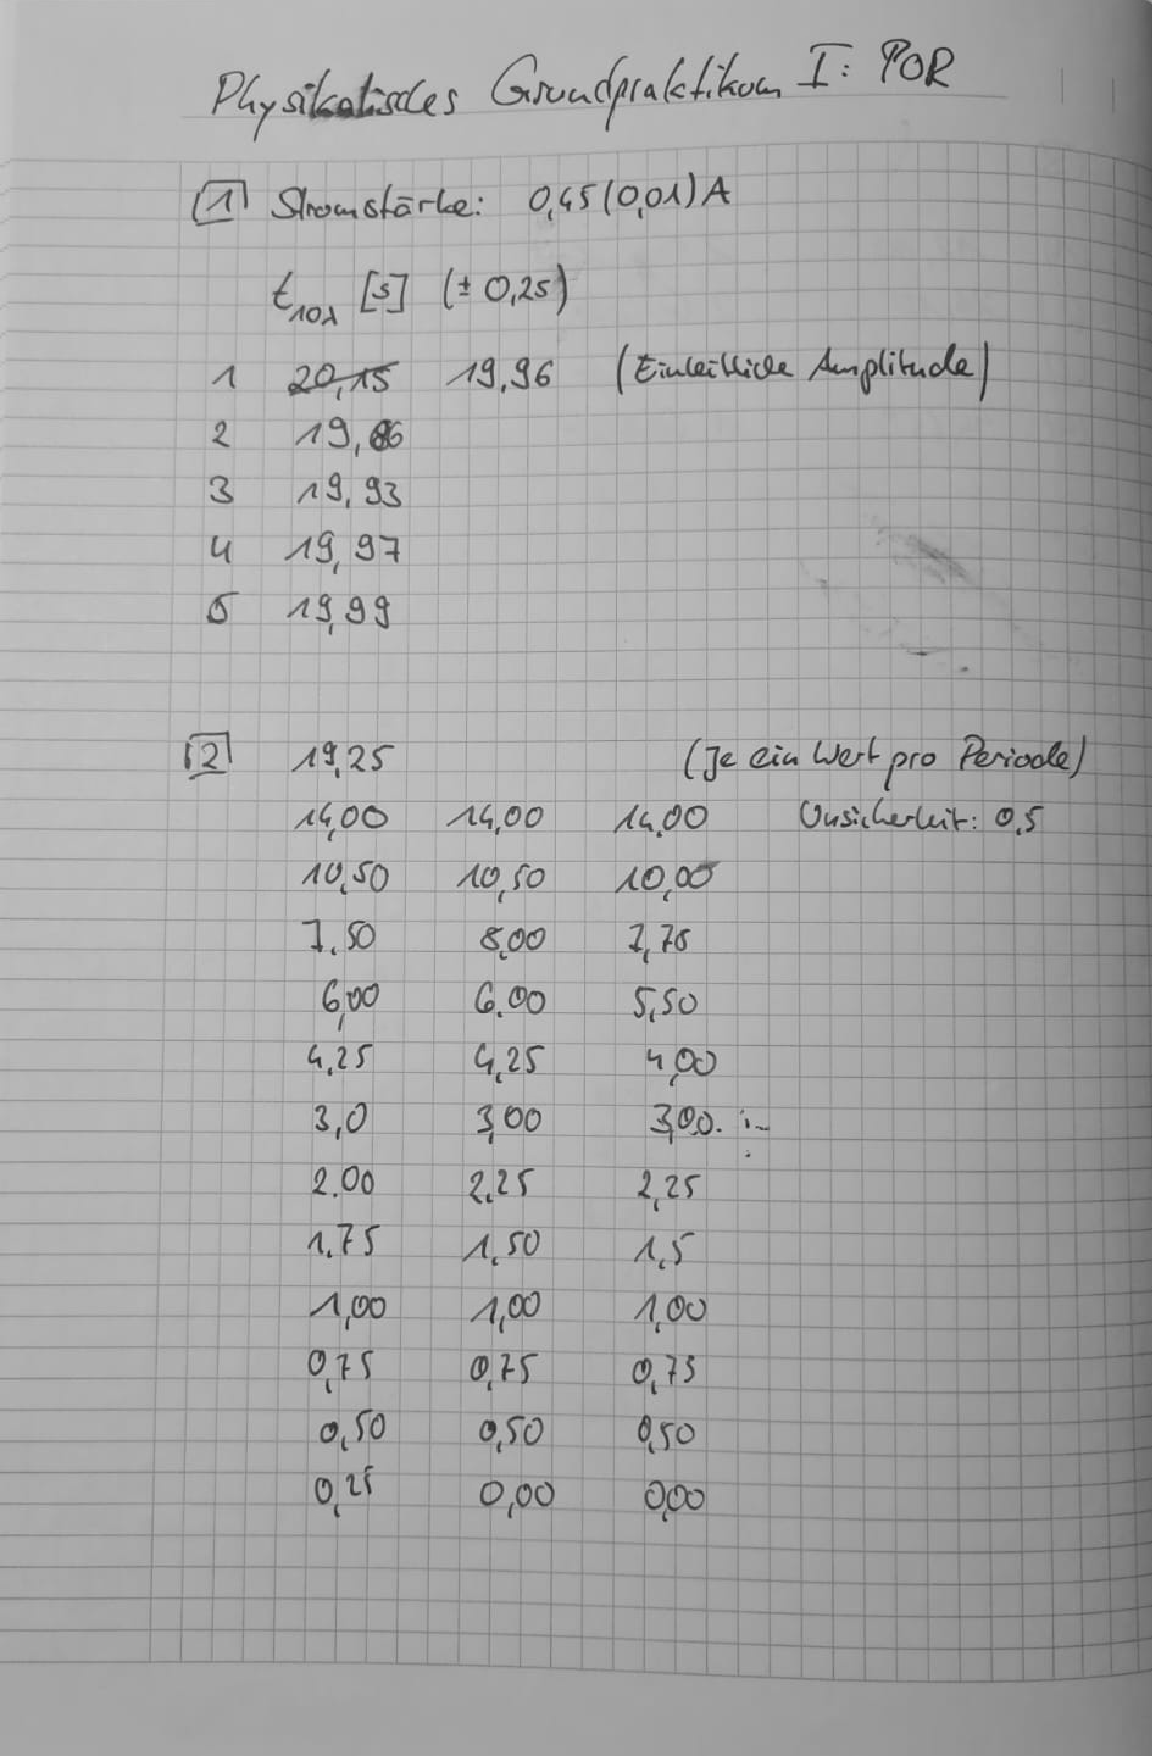
\includepdf[pages=-]{Protokoll.pdf}
\end{document}
